\documentclass{llncs}

\usepackage[utf8]{inputenc}
\usepackage[T1]{fontenc}
\usepackage{mathptmx}
\usepackage{graphicx}
\usepackage{amsmath,amsfonts,amssymb}
\usepackage{booktabs}
\usepackage{hyperref}
\usepackage[authoryear,round]{natbib}
\usepackage{url}

\renewcommand{\bibsection}{\section*{Referencias}}

% APA 7: sin numerar, sin sangría francesa
\makeatletter
\renewenvironment{thebibliography}[1]{%
  \bibsection
  \list{}{%
    \setlength{\labelwidth}{0pt}%
    \setlength{\labelsep}{0pt}%
    \setlength{\leftmargin}{0pt}%
    \setlength{\itemindent}{0pt}%
    \setlength{\itemsep}{4pt plus 1pt}%
    \def\makelabel##1{}%
  }%
  \sloppy
  \sfcode`\.\@m
}{\endlist}
\makeatother

\begin{document}

\title{Hacia la implementación de un modelo neuronal de integración
multisensorial de inferencia probabilística con dinámicas corticales
realistas}

\author{Franco Molina
\email{franco.molina13@mi.unc.edu.ar}
\and Renato Paredes Venero
\email{renato.paredes@mi.unc.edu.ar}
\and Juan B. Cabral
\email{jbcabral@unc.edu.ar}}

\institute{Facultad de Matemática, Astronomía, Física y Computación,
Universidad Nacional de Córdoba}

\maketitle

\renewcommand{\abstractname}{Resumen}
\begin{abstract}
La integración multisensorial, el proceso mediante el cual el
cerebro combina información de distintas modalidades sensoriales,
constituye un área fundamental de la neurociencia computacional. Los
modelos existentes presentan una brecha significativa: aquellos que
capturan la arquitectura funcional de la integración multisensorial
carecen de dinámicas corticales realistas, mientras que los modelos
con dinámicas biológicamente plausibles están limitados al
procesamiento unimodal. Este trabajo aborda el primer paso hacia dicha fusión mediante la
implementación del modelo unimodal de \citet{echeveste2020cortical},
que opera sobre una única modalidad sensorial (visual), dentro del
framework Scikit-NeuroMSI, una plataforma de código abierto en Python
para la modelización neurocomputacional de la integración
multisensorial. Al integrar este modelo unimodal en un framework
multimodal, se sientan las bases para su futura extensión hacia el
procesamiento de múltiples modalidades sensoriales. La
reimplementación, desde Python/OCaml hacia Python/JAX, fue validada
alcanzando equivalencia numérica con errores del orden de
$10^{-15}$. Como contribuciones adicionales, se
desarrollaron dos módulos de soporte para gestión de parámetros
pre-entrenados y para modelos generativos, posicionando esta
implementación como base técnica fundamental para la futura
investigación planteada que combina dinámicas corticales realistas
con integración multisensorial.
\keywords{inferencia probabilística -- muestreo neuronal --
redes recurrentes -- integración multisensorial -- Scikit-NeuroMSI}
\end{abstract}

\begin{center}
\Large\bfseries
Towards the implementation of a neural model of multisensory
integration for probabilistic inference with realistic cortical
dynamics
\end{center}

\renewcommand{\abstractname}{Abstract}
\begin{abstract}
Multisensory integration, the process by which the brain combines
information from different sensory modalities, constitutes a
fundamental area of computational neuroscience. Existing models
present a significant gap: those that capture the functional
architecture of multisensory integration lack realistic cortical
dynamics, while models with biologically plausible dynamics are
limited to unimodal processing. This work addresses the first step towards bridging this gap through
the implementation of the unimodal model of
\citet{echeveste2020cortical}, which operates on a single sensory
modality (visual), within the Scikit-NeuroMSI framework, an
open-source Python platform for neurocomputational modeling of
multisensory integration. By integrating this unimodal model into a
multimodal framework, the foundations are laid for its future
extension towards multisensory processing. The reimplementation, from
Python/OCaml to Python/JAX, was validated
through four complementary levels: unit testing of individual
components, function-by-function comparison against the original
code achieving numerical equivalence with errors on the order of
$10^{-15}$, robustness analysis of the two-stage training procedure
across 100 independent runs, and replication of the central
simulations of the original article. The implemented network
faithfully reproduces probabilistic inference via sampling,
exhibiting characteristic emergent properties such as
stimulus-modulated variability (quenching), inhibitory transients,
and gamma-band oscillations whose peak frequency increases with
stimulus contrast. As additional contributions, two support modules
were developed for managing pre-trained parameters and generative
models, positioning this implementation as a fundamental technical
foundation for the proposed future research combining realistic
cortical dynamics with multisensory integration.
\keywords{probabilistic inference -- neural sampling --
recurrent networks -- multisensory integration -- Scikit-NeuroMSI}
\end{abstract}

\section{Introducción}

La integración multisensorial es un proceso neuronal fundamental
mediante el cual el cerebro combina información proveniente de
distintas modalidades sensoriales para generar representaciones más
robustas y confiables del entorno. Este fenómeno, documentado
extensamente desde los estudios pioneros en el colículo superior
\citep{stein2012new}, constituye una de las capacidades más notables
del sistema nervioso.

Diversos enfoques computacionales han buscado capturar los mecanismos
subyacentes a esta integración. Entre estos desarrollos, dos trabajos
resultan particularmente relevantes por representar enfoques
complementarios al problema. Por un lado, el modelo de
\citet{cuppini2017biologically} aborda la integración audiovisual
mediante una arquitectura de tres capas jerárquicas que reproduce
fenómenos experimentales como el efecto ventrílocuo. Sin embargo, al
utilizar modelos de tasa deterministas, este enfoque no captura la
variabilidad ni las dinámicas oscilatorias características de la
actividad cortical real. Por otro lado, el modelo de
\citet{echeveste2020cortical} demuestra que redes neuronales con
restricciones biológicas pueden implementar inferencia probabilística
mediante muestreo estocástico, exhibiendo propiedades emergentes como
oscilaciones gamma y variabilidad modulada por el estímulo; no
obstante, este modelo está restringido al procesamiento unimodal.

Esta situación revela una brecha significativa: los modelos que
capturan la arquitectura funcional de la integración multisensorial
carecen de dinámicas corticales realistas, mientras que aquellos con
dinámicas biológicamente plausibles están limitados al procesamiento
unimodal. La visión a largo plazo que motiva este trabajo es el
desarrollo de modelos que combinen la arquitectura multimodal del
enfoque de Cuppini con las dinámicas corticales del modelo de
Echeveste. Alcanzar esta visión, sin embargo, requiere primero sentar
bases técnicas sólidas.

El presente trabajo representa el primer paso en esta dirección
mediante la implementación del modelo de Echeveste dentro del
framework Scikit-NeuroMSI \citep{paredes2025scikit}, una plataforma
de código abierto en Python\footnote{\url{https://www.python.org/}}
diseñada específicamente para la modelización neurocomputacional de
la integración multisensorial. Esta implementación incluye la
arquitectura de red con poblaciones excitatorias e inhibitorias, el
modelo generativo que define el problema de inferencia, y el
procedimiento de entrenamiento para muestreo.

\section{El modelo de Echeveste}

El trabajo de \citet{echeveste2020cortical} parte de restricciones
biológicas sobre la dinámica de circuitos corticales para demostrar
que redes neuronales recurrentes pueden ser optimizadas para
implementar inferencia probabilística basada en muestreo. Se trata
de un modelo \emph{unimodal}: opera exclusivamente sobre estímulos
visuales, modelando una hipercolumna de la corteza visual primaria
donde las neuronas responden a la orientación de bordes en el campo
visual, sin abordar la integración de múltiples modalidades
sensoriales. A continuación, se describen los componentes centrales.

\subsection{Marco teórico: muestreo como inferencia}

La percepción puede entenderse como inferencia bayesiana sobre las
causas latentes de las observaciones sensoriales. Dado un estímulo
$\mathbf{x}$, el cerebro busca inferir las variables latentes
$\mathbf{y}$ que lo generaron, caracterizadas por la distribución
posterior $P(\mathbf{y}|\mathbf{x})$. La hipótesis del \emph{muestreo
neuronal} propone que, en lugar de representar esta distribución
analíticamente, el cerebro la representa mediante muestras
temporales, de modo que la distribución empírica de actividades a lo
largo del tiempo aproxima la posterior \citep{echeveste2020cortical}.

\subsection{El modelo generativo (GSM)}

Para especificar el problema computacional objetivo, se adopta el
\emph{modelo de mezcla de escala gaussiana} (\textsc{gsm}), un modelo
generativo que captura las estadísticas de parches de imágenes
naturales. Un parche $\mathbf{x} \in \mathbb{R}^{N_x}$ se genera
como:

\begin{equation}
\mathbf{x} = z \cdot \mathbf{A}\mathbf{y} + \boldsymbol{\epsilon},
\qquad \mathbf{y} \sim \mathcal{N}(\mathbf{0}, \mathbf{C})
\label{eq:gsm}
\end{equation}

donde $\mathbf{y}$ son variables latentes, $\mathbf{A}$ es la matriz
de campos proyectivos tipo Gabor, $z$ es el contraste, y
$\boldsymbol{\epsilon}$ es ruido sensorial. Bajo el \textsc{gsm}, la
posterior sobre las variables latentes dado un parche y un contraste
conocido tiene forma gaussiana, con media y covarianza que dependen
de $z$ de manera que a mayor contraste, menor incertidumbre.

\subsection{Dinámica neuronal y arquitectura}

El modelo implementa una \emph{red supralineal estabilizada}
(\textsc{ssn}) que modela una hipercolumna de V1, con
$N_E = N_I = 50$ neuronas organizadas en una topología de anillo
según sus orientaciones preferidas. La dinámica de cada neurona está
gobernada por:

\begin{equation}
\tau_i \frac{du_i}{dt} = -u_i(t) + h_i(t) + \sum_j W_{ij} r_j(t) +
\eta_i(t)
\label{eq:ssn}
\end{equation}

donde $u_i$ es el potencial de membrana, $h_i$ la entrada
feedforward, $W_{ij}$ los pesos recurrentes, $r_j = k[u_j]_+^n$ la
tasa de disparo con no linealidad supralineal, y $\eta_i$ ruido
gaussiano correlacionado. La conectividad $\mathbf{W}$ se parametriza
de forma rotacionalmente simétrica, reduciendo los grados de libertad
de $N^2 = 10{,}000$ a solo 15 parámetros totales que respetan el
principio de Dale.

\subsection{Entrenamiento para muestreo}

A diferencia de enfoques tradicionales, el objetivo es que la
\emph{distribución} de respuestas de la red coincida con la posterior
del modelo generativo. Para ello se minimiza una función de costo que
penaliza diferencias entre los momentos de la red y los momentos
objetivo de la posterior, junto con un término de \emph{slowness} que
incentiva independencia temporal entre muestras:

\begin{equation}
\mathcal{F} = \sum_\alpha \left( \epsilon_{\mu} \phi_{\mu}^{(\alpha)}
+ \epsilon_{\sigma} \phi_{\sigma}^{(\alpha)} + \epsilon_{\Sigma}
\phi_{\Sigma}^{(\alpha)} + \epsilon_{\text{slow}}
\phi_{\text{slow}}^{(\alpha)} \right)
\label{eq:costo}
\end{equation}

El procedimiento de optimización se realiza en dos etapas: una
estocástica con \textsc{adam} (250 iteraciones, $N_{\text{trial}} =
50$) y una determinística con \textsc{l-bfgs-b} que emplea el método
\emph{Assumed Density Filtering} (\textsc{adf}) para obtener
gradientes exactos bajo una aproximación gaussiana de la distribución
conjunta espacio-temporal.

\section{Implementación}

Con el conocimiento del modelo de Echeveste, procedemos a describir
en detalle las decisiones de diseño, los desafíos que enfrentamos y
las contribuciones realizadas al framework Scikit-NeuroMSI.

\subsection{Arquitectura del código}

La implementación se organizó en cinco módulos dentro del paquete
\texttt{skneuromsi/\-neural/\-echeveste2020}, separando
responsabilidades según el principio de responsabilidad única:
\texttt{\_model.py} con la clase principal \texttt{Echeveste2020};
\texttt{\_training.py} con las funciones de entrenamiento basadas en
diferenciación automática; \texttt{\_gsm.py} con el modelo
generativo; \texttt{\_visualization.py} con herramientas de análisis
para dinámicas temporales; y \texttt{\_data\_loader.py} con el acceso
a parámetros pre-entrenados. La clase \texttt{Echeveste2020} hereda
de \texttt{SKNMSIMethodABC}, lo que garantiza compatibilidad con las
herramientas del framework.

\subsection{Reimplementación en JAX}

Uno de los desafíos inesperados del trabajo fue descubrir que el
código de entrenamiento original se encontraba implementado en
OCaml\footnote{\url{https://ocaml.org/}}, un lenguaje funcional
atípico para el desarrollo actual de modelos de redes neuronales. En
comunicación personal con el autor original, pudimos comprender que,
al momento en que se desarrolló el modelo, las herramientas de
diferenciación automática hoy consideradas estándar no existían o no
habían alcanzado la madurez necesaria para este tipo de
aplicaciones. Sin embargo, esta decisión técnica, perfectamente
razonable en su contexto original, dejó el código en un estado de
difícil acceso para la comunidad científica actual.

La reimplementación en JAX\footnote{\url{https://docs.jax.dev/}}
constituyó, por tanto, no solo una traducción de código sino una
actualización tecnológica sustancial. JAX fue la elección natural por
varias razones: su paradigma de programación funcional guarda
afinidad conceptual con OCaml, lo que facilitó la traducción de las
estructuras algorítmicas; ya se encontraba integrado en
Scikit-NeuroMSI como dependencia para otros componentes; y ofrece
compilación \emph{Just-In-Time} mediante \textsc{xla} que optimiza
automáticamente las operaciones para el hardware disponible, junto
con soporte transparente para ejecución en \textsc{gpu}.

\subsection{Módulos de soporte}

Además de la implementación central, el trabajo contribuyó
estructurando dos módulos completamente nuevos al framework. El
módulo \texttt{data} fue implementado como infraestructura para
gestionar el acceso a datos pre-entrenados, exportando las clases
\texttt{EchevesteDataLoader} y \texttt{GSMDataLoader} que
proporcionan acceso estructurado a la matriz de conectividad
optimizada, la matriz de covarianza de ruido, los parámetros de la
transformación de entrada, y los componentes del modelo generativo.

El módulo \texttt{generative} representa una extensión conceptual
significativa del framework, introduciendo por primera vez la
capacidad de definir modelos generativos que especifican el problema
de inferencia. Actualmente contiene la clase \texttt{GSM}, aunque la
arquitectura fue diseñada con extensibilidad en mente: futuros
trabajos podrían agregar otros modelos generativos siguiendo la misma
interfaz.

\subsection{Modos de simulación}

La implementación soporta dos modos de simulación. El \emph{modo de
fase única} mantiene el estímulo presente durante toda la simulación
y replica las condiciones utilizadas durante el entrenamiento. El
\emph{modo de tres fases} divide la simulación en períodos
pre-estímulo, estímulo y post-estímulo, permitiendo estudiar
fenómenos dinámicos como los transitorios al \emph{onset} y las
oscilaciones moduladas por el estímulo. El modo de tres fases soporta
opcionalmente \emph{delays} por neurona en las transiciones,
modelando la variabilidad temporal con que diferentes neuronas
reciben la señal de entrada.

\section{Resultados}

La validación de la implementación se realizó en cuatro niveles
complementarios: pruebas unitarias, validación función por función,
análisis del procedimiento de entrenamiento, y reproducción de las
simulaciones centrales del artículo original.

\subsection{Validación función por función}

Se realizó una validación exhaustiva comparando cada función de
nuestra implementación con su equivalente en el código original. La
metodología consistió en generar $N = 10{,}000$ muestras aleatorias
para cada función, ejecutar ambas implementaciones con inputs
idénticos, y calcular el error máximo absoluto. La
Tabla~\ref{tab:validation} presenta el resumen por categoría.

\begin{table}[!ht]
\centering
\caption{Validación función por función contra el código original de
Echeveste ($N = 10{,}000$ muestras por función).}
\label{tab:validation}
\begin{tabular}{clc}
\toprule
\textbf{\#} & \textbf{Categoría} & \textbf{Error máximo} \\
\midrule
1 & Distribución Normal & $0.00$ \\
2 & Activación Neuronal & $0.00$ \\
3 & Momentos $\nu$, $\gamma$ & $7.11 \times 10^{-15}$ \\
4 & Evolución Temporal & $0.00$ \\
5 & Conectividad Paramétrica & $0.00$ \\
6 & Ruido Ornstein--Uhlenbeck & $1.11 \times 10^{-16}$ \\
7 & GSM Posterior & $0.00$ \\
8 & Funciones Auxiliares & $0.00$ \\
\bottomrule
\end{tabular}
\end{table}

Los resultados demuestran que las 25 funciones evaluadas producen
resultados numéricamente equivalentes, con errores máximos del orden
de la precisión de punto flotante de doble precisión
($\sim 10^{-15}$). Los errores no nulos observados corresponden
exactamente al épsilon de máquina IEEE 754
($\epsilon \approx 2.22 \times 10^{-16}$), y surgen de diferencias en
el orden de operaciones aritméticas entre implementaciones, no de
discrepancias algorítmicas.

\subsection{Convergencia del entrenamiento}

Para evaluar la robustez del procedimiento, se ejecutaron 100
corridas independientes partiendo de condiciones iniciales
aleatorias. Las amplitudes de conectividad convergieron
consistentemente hacia los valores de referencia, con coeficientes de
variación menores al 10\% en la mayoría de los casos. Los parámetros
de la transformación de entrada ($\alpha_h$, $\beta_h$, $\gamma_h$)
exhibieron errores relativos menores al 5\% respecto a los valores
reportados. El exponente $\gamma_h \approx 2$ resulta particularmente
notable: su proximidad al exponente supralineal $n = 2$ sugiere una
consistencia en el procesamiento no lineal a través del modelo, que
emerge de la optimización sin ser impuesta \emph{a priori}.

Los parámetros del ruido revelaron un fenómeno interesante: las
desviaciones estándar $\sigma_E$ y $\sigma_I$ exhibieron mayor
variabilidad entre corridas, pero la proporción $\sigma_E/\sigma_I$
se mantuvo aproximadamente constante, indicando la existencia de una
familia de soluciones equivalentes en el espacio de parámetros.

\subsection{Actividad poblacional y patrones de disparo}

La validación de las propiedades de inferencia se inicia verificando
que la red reproduce los patrones de actividad poblacional reportados
en el artículo original. La Figura~\ref{fig:fig2a} muestra los
potenciales de membrana excitatorios $u_E$ en función del tiempo y la
orientación para los casos extremos de contraste.

\begin{figure}[!ht]
    \centering
    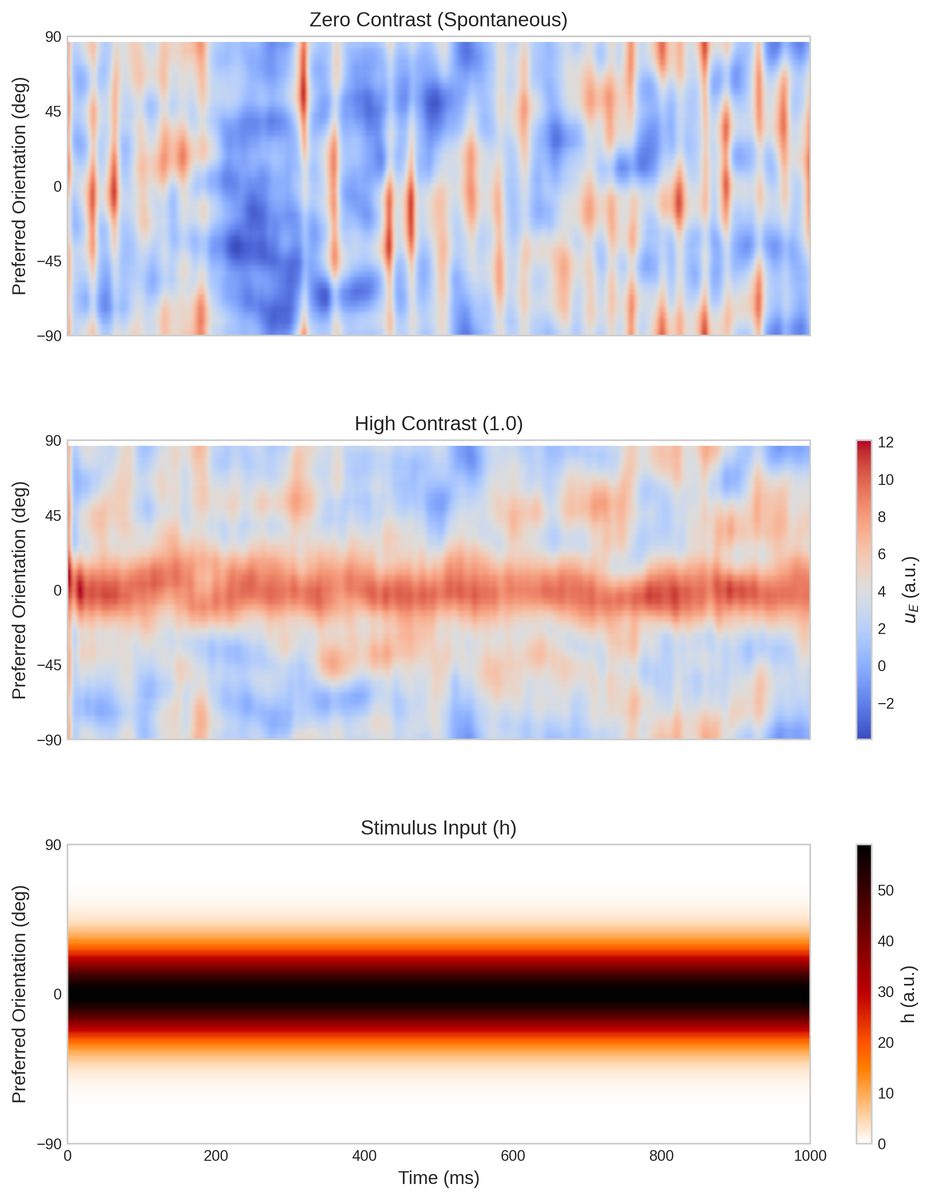
\includegraphics[width=0.95\textwidth]{08_resultados/figures_small/fig2a_population_activity_open.png}
    \caption{Actividad poblacional de potenciales de membrana
    excitatorios. Primer panel: contraste $z = 0$ (actividad
    espontánea). Panel central: contraste $z = 1$ (estimulación
    máxima). Último panel: entrada feedforward $\mathbf{h}$
    correspondiente al contraste máximo. El eje vertical representa
    la orientación preferida de cada neurona ($-90°$ a $90°$); el
    eje horizontal, el tiempo.}
    \label{fig:fig2a}
\end{figure}

En ausencia de estímulo, la actividad fluctúa alrededor de valores
bajos con distribución espacial aproximadamente uniforme, reflejando
el ruido de proceso $\boldsymbol{\eta}(t)$ filtrado por la dinámica
recurrente. Con contraste máximo, la presencia de un estímulo con
orientación dominante en $0°$ induce un incremento de actividad
centrado en las neuronas con orientación preferida cercana a esta
dirección.

Una representación complementaria se obtiene mediante \emph{raster
plots}, donde cada marca vertical representa un potencial de acción.
La Figura~\ref{fig:raster} compara la actividad espontánea con la
evocada por estímulo. Notablemente, las neuronas inhibitorias (rojo)
exhiben tasas de disparo superiores a las excitatorias (azul) en
ambas condiciones, comportamiento consistente con la dinámica de
redes supralineales estabilizadas donde la inhibición debe ser
suficientemente fuerte para prevenir la excitación descontrolada
inducida por el estímulo.

\begin{figure}[!ht]
    \centering
    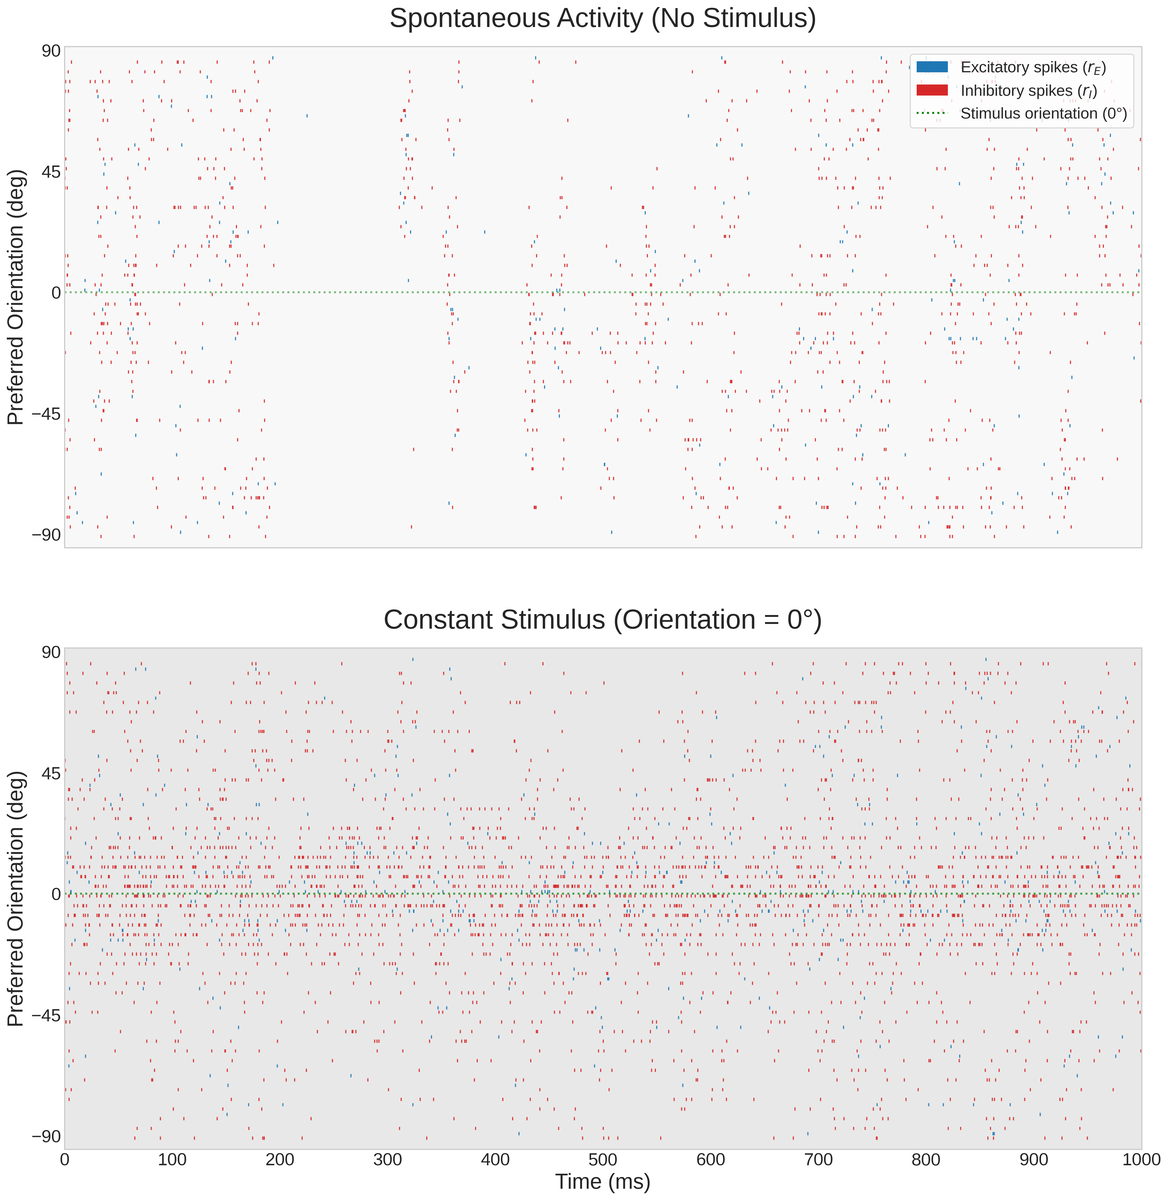
\includegraphics[width=0.95\textwidth]{08_resultados/figures_small/fig_raster_comparison.png}
    \caption{Raster plot comparando actividad espontánea y evocada.
    Cada marca vertical representa un spike. Neuronas excitatorias en
    azul, inhibitorias en rojo. Panel superior: actividad espontánea
    sin estímulo, mostrando disparos dispersos distribuidos
    uniformemente. Panel inferior: actividad durante presentación de
    estímulo a $0°$ (línea punteada verde) de alto contraste $z=1.0$,
    con disparos concentrados alrededor de la orientación del
    estímulo.}
    \label{fig:raster}
\end{figure}

\subsection{Estructura de correlaciones poblacionales}

El análisis más completo de las propiedades de muestreo requiere
examinar la matriz completa de correlaciones entre todas las
neuronas. La Figura~\ref{fig:correlation} presenta esta comparación,
mostrando que las matrices exhiben la estructura característica de la
topología de anillo.

\begin{figure}[!ht]
    \centering
    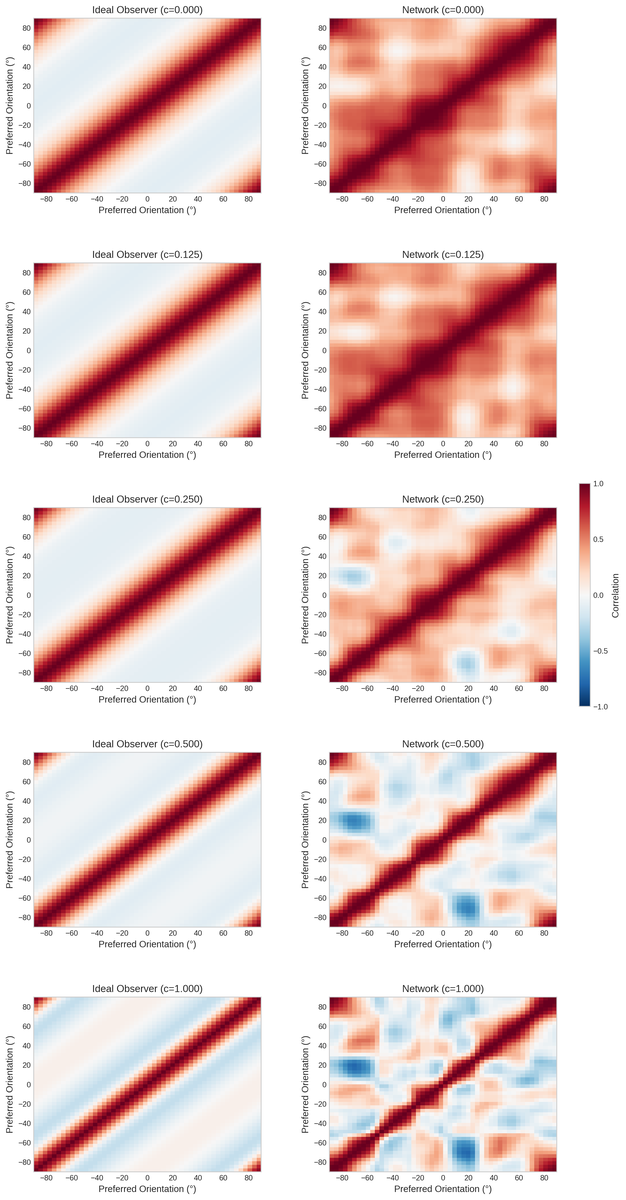
\includegraphics[width=0.6\textwidth]{08_resultados/figures_small/Fig2d_correlation_matrices.png}
    \caption{Matrices de correlación de Pearson entre potenciales de
    membrana excitatorios. Columna izquierda: observador ideal
    (\textsc{gsm}). Columna derecha: red neuronal (\textsc{ssn}).
    Cada fila corresponde a un nivel de contraste diferente.}
    \label{fig:correlation}
\end{figure}

La diagonal principal muestra máxima correlación, y a medida que nos
alejamos de la diagonal, la correlación decae gradualmente,
reflejando que neuronas con orientaciones preferidas más distantes
están menos correlacionadas. La estructura se modifica con el
contraste de manera consistente entre el observador ideal y la red:
para contraste cero, las correlaciones están determinadas
principalmente por el prior del \textsc{gsm}, mientras que con el
aumento del contraste, la estructura refleja progresivamente más la
información del estímulo. Calculando la correlación de Pearson
elemento por elemento entre ambas matrices, se obtienen valores
superiores a 0.95 para todos los niveles de contraste, confirmando
que la red no solo reproduce los momentos marginales correctos sino
también la estructura completa de dependencias.

\subsection{Dinámicas emergentes}

Más allá de reproducir los momentos estadísticos correctos, el modelo
de Echeveste se distingue por exhibir un conjunto de propiedades
dinámicas que emergen como consecuencia del objetivo de muestreo, sin
ser explícitamente impuestas durante el entrenamiento. Nuestra
implementación preserva estas características, las cuales se
describen a continuación.

\textbf{Variabilidad modulada por el estímulo.} La varianza de las
respuestas neuronales decrece con el contraste del estímulo,
fenómeno conocido como \emph{quenching} y observado experimentalmente
en corteza visual de primates \citep{echeveste2020cortical}. Este
comportamiento puede cuantificarse mediante el factor de Fano,
$F = \text{Var}[r] / \mathbb{E}[r]$, cuya reducción sistemática con
el contraste verificamos en nuestras simulaciones: para $z = 0$ se
encuentra en el rango $1.0$--$1.2$, mientras que para $z = 1$ decrece
hacia valores en $0.6$--$0.8$. La reducción es particularmente
pronunciada para las neuronas cuya orientación preferida coincide con
la del estímulo, reflejando directamente las propiedades de la
posterior del \textsc{gsm}, donde mayor contraste implica menor
incertidumbre.

\textbf{Transitorios inhibitorios.} Al inicio de un estímulo, la
inhibición domina transitoriamente sobre la excitación, generando
sobrepicos (\emph{overshoots}) en las tasas de disparo poblacionales
seguidos de adaptación hacia el estado estacionario. Lejos de
constituir defectos del modelo, estos transitorios cumplen un rol
funcional al acelerar la convergencia de las muestras hacia la
distribución estacionaria correcta, reduciendo el tiempo de
\emph{burn-in}. El análisis teórico de \citet{echeveste2020cortical}
muestra que la trayectoria óptima que minimiza el error de estimación
en una ventana temporal finita debe exhibir sobrepicos cuya magnitud
escala con el valor objetivo, predicción que validaron mediante
registros experimentales en V1 de mono despierto.

\textbf{Oscilaciones gamma.} La actividad de la red exhibe
oscilaciones en el rango gamma (30--80 Hz), detectables tanto en
autocorrelogramas de neuronas individuales como en el potencial de
campo local (\textsc{lfp}) simulado, calculado como el promedio de
los potenciales de membrana excitatorios. La frecuencia pico aumenta
con el contraste del estímulo, comportamiento que verificamos en
nuestras simulaciones mediante análisis espectral de Welch sobre el
\textsc{lfp}: la frecuencia pico se desplaza desde $\sim 32$ Hz para
contraste bajo hasta $\sim 56$ Hz para contraste máximo. Estas
oscilaciones implementan una forma de muestreo fuera del equilibrio
que acelera la exploración del espacio de estados: a diferencia de
algoritmos de muestreo clásicos como Langevin (cuya dinámica
reversible limita la velocidad de mezcla), las trayectorias
oscilatorias de la red optimizada permiten que muestras consecutivas
cubran una región más amplia del espacio, alcanzando convergencia un
orden de magnitud más rápido. Este resultado es particularmente
significativo dado que las oscilaciones gamma se observan
consistentemente en registros electrofisiológicos de V1 de primates,
sugiriendo que podrían constituir un subproducto funcional del
cómputo probabilístico más que un epifenómeno.

\section{Conclusiones y trabajo a futuro}

En este trabajo llevamos a cabo la implementación completa del
modelo de \citet{echeveste2020cortical} dentro del framework
Scikit-NeuroMSI, estableciendo las bases técnicas necesarias para
futuras investigaciones que combinen dinámicas corticales realistas
con integración multisensorial. La reimplementación, que requirió
una traducción completa desde OCaml hacia Python utilizando JAX para
diferenciación automática, resultó en una implementación moderna
compatible con el ecosistema actual, con soporte transparente para
aceleración en \textsc{gpu} y una arquitectura modular que facilita
futuras extensiones.

La validación se realizó en múltiples niveles complementarios. La
verificación función por función demostró equivalencia numérica
exacta con errores del orden de la precisión de punto flotante. Las
pruebas del procedimiento de entrenamiento confirmaron que los
parámetros optimizados convergen hacia valores comparables a los de
referencia. Las simulaciones replicaron las figuras centrales del
artículo original, verificando que la red implementada reproduce
correctamente las propiedades de inferencia probabilística mediante
muestreo y las dinámicas temporales características, incluyendo
oscilaciones gamma cuya frecuencia aumenta con el contraste.

Como contribuciones adicionales al framework, se desarrollaron los
módulos \texttt{data} (infraestructura para gestionar parámetros
pre-entrenados) y \texttt{generative} (que introduce por primera vez
modelos generativos como el \textsc{gsm}, diseñado con extensibilidad
en mente).

La dirección más prometedora para trabajo futuro es la integración
del modelo de Echeveste con el modelo de Cuppini ya implementado en
Scikit-NeuroMSI. Sin embargo, esta fusión requiere resolver
adaptaciones fundamentales que van más allá de una integración
directa. La diferencia más significativa reside en el dominio de
representación neuronal: las neuronas del modelo de Echeveste están
organizadas según su \emph{orientación preferida} de estímulos
visuales (topología de anillo en una hipercolumna de V1), mientras
que las neuronas del modelo de Cuppini están organizadas
topográficamente según la \emph{posición espacial} en el campo visual
y auditivo. Esta diferencia implica que la conectividad, las
funciones de sintonización y el modelo generativo subyacente operan
sobre espacios de características distintos. Entre las principales
adaptaciones necesarias se encuentran: (i) rediseñar la topología de
la red para que las neuronas respondan a posición espacial en lugar
de orientación, lo cual modifica la parametrización circulante de la
matriz de conectividad; (ii) reformular el modelo generativo,
reemplazando el \textsc{gsm} basado en filtros de Gabor orientados
por uno que capture las estadísticas de localización espacial de
estímulos audiovisuales; (iii) extender la arquitectura de una red
unimodal a múltiples capas interconectadas (auditiva, visual y
multisensorial) preservando las dinámicas de muestreo estocástico;
y (iv) incorporar mecanismos de inferencia causal que determinen si
estímulos de distintas modalidades provienen de una causa común o de
fuentes independientes. A diferencia de los modelos deterministas de
tasa existentes, un modelo así generaría señales de \textsc{lfp}
simuladas con oscilaciones emergentes en bandas fisiológicamente
relevantes, lo que abriría la posibilidad de modelar directamente
las dinámicas oscilatorias cerebrales asociadas a la integración
multisensorial y contrastarlas con registros electrofisiológicos
reales.

Otras líneas complementarias incluyen la extensión de la validación
experimental del modelo mediante réplicas de análisis como los de
\citet{banyai2019stimulus}, la implementación de otros modelos
generativos dentro del módulo \texttt{generative} para investigar
sistemáticamente cómo las propiedades emergentes del circuito
dependen del problema de inferencia que la red debe resolver, y la
formalización de la separación entre generación de estímulos y
modelos neuronales, como propone \citet{paredes2025scikit}.

\section{Agradecimientos}

Agradezco al Dr. Rodrigo Echeveste por su disposición a responder
consultas sobre el modelo original. Finalmente, agradezco a la
Facultad de Matemática, Astronomía, Física y Computación de la
Universidad Nacional de Córdoba, en cuyo marco se desarrolló esta
investigación.

\begin{thebibliography}{}

\bibitem[Bányai et al.(2019)]{banyai2019stimulus}
Bányai, M., Lazar, A., Klein, L., Klon-Lipok, J., Stippinger, M.,
Singer, W., \& Orbán, G. (2019). Stimulus complexity shapes response
correlations in primary visual cortex. \emph{Proceedings of the
National Academy of Sciences}, \emph{116}(7), 2723--2732.

\bibitem[Berkes et al.(2011)]{berkes2011spontaneous}
Berkes, P., Orbán, G., Lengyel, M., \& Fiser, J. (2011). Spontaneous
cortical activity reveals hallmarks of an optimal internal model of
the environment. \emph{Science}, \emph{331}(6013), 83--87.

\bibitem[Cuppini et al.(2017)]{cuppini2017biologically}
Cuppini, C., Shams, L., Magosso, E., \& Ursino, M. (2017). A
biologically inspired neurocomputational model for audiovisual
integration and causal inference. \emph{European Journal of
Neuroscience}, \emph{46}(9), 2481--2498.

\bibitem[Echeveste et al.(2020)]{echeveste2020cortical}
Echeveste, R., Aitchison, L., Hennequin, G., \& Lengyel, M. (2020).
Cortical-like dynamics in recurrent circuits optimized for
sampling-based probabilistic inference. \emph{Nature Neuroscience},
\emph{23}(9), 1138--1149.

\bibitem[Gerstner and Kistler(2002)]{gerstner2002spiking}
Gerstner, W., \& Kistler, W. M. (2002). \emph{Spiking neuron models:
Single neurons, populations, plasticity}. Cambridge University Press.

\bibitem[Haefner et al.(2016)]{haefner2016perceptual}
Haefner, R. M., Berkes, P., \& Fiser, J. (2016). Perceptual
decision-making as probabilistic inference by neural sampling.
\emph{Neuron}, \emph{90}(3), 649--660.

\bibitem[Körding et al.(2007)]{kording2007causal}
Körding, K. P., Beierholm, U., Ma, W. J., Quartz, S., Tenenbaum,
J. B., \& Shams, L. (2007). Causal inference in multisensory
perception. \emph{PLoS One}, \emph{2}(9), e943.

\bibitem[Paredes et al.(2025)]{paredes2025scikit}
Paredes, R., Cabral, J. B., \& Seriès, P. (2025). Scikit-NeuroMSI: A
generalized framework for modeling multisensory integration.
\emph{Neuroinformatics}, \emph{23}(3), 40.

\bibitem[Stein(2012)]{stein2012new}
Stein, B. E. (2012). \emph{The new handbook of multisensory
processing}. MIT Press.

\bibitem[Ursino et al.(2017)]{ursino2017multisensory}
Ursino, M., Cuppini, C., \& Magosso, E. (2017). Multisensory Bayesian
inference depends on synapse maturation during training: Theoretical
analysis and neural modeling implementation. \emph{Neural
Computation}, \emph{29}(3), 735--782.

\end{thebibliography}

\end{document}
